\documentclass[a4paper,10pt,english]{article}
\usepackage[utf8]{inputenc}
%\bibliography{references.bib}
% Standard stuff
\usepackage{amsmath,amssymb,graphicx,babel,varioref,verbatim,amsfonts,float}
\usepackage[a4paper, total={6in, 8in}]{geometry}
%\usepackage{biblatex}
\usepackage{csquotes}
\usepackage[round]{natbib}
\bibliographystyle{plainnat}
\usepackage[bottom]{footmisc}
\usepackage{multirow}
\usepackage{adjustbox}
\usepackage{tabularx}
\usepackage[font=small]{caption}
\usepackage{booktabs} %nicer tables
%\usepackage{subcaption}

% arrows upuparrows downuparrows
\newcommand{\updownarrows}{\uparrow\mathrel{\mspace{-1mu}}\downarrow}
\newcommand{\downuparrows}{\downarrow\mathrel{\mspace{-1mu}}\uparrow}
\renewcommand{\upuparrows}{\uparrow\uparrow}
\renewcommand{\downdownarrows}{\downarrow\downarrow}

\usepackage{mathrsfs} % fancy lettering
\newcolumntype{Y}{>{\centering\arraybackslash}X} % centered columns with textwidth
% colors in text
\usepackage[usenames,dvipsnames,svgnames,table]{xcolor}
% Hyper refs
\usepackage[colorlinks,linkcolor=black,citecolor=black]{hyperref}

% Document formatting
\setlength{\parindent}{2em}
\setlength{\parskip}{1.5mm}

\def\code#1{\texttt{#1}} % make single word look like code, comand \code{...}
%Equation formatting
\usepackage{physics}	% For derivative fraction symbol, partial and total
\newcommand\numberthis{\addtocounter{equation}{1}\tag{\theequation}} % number certain equations in align*
\newcommand{\matr}[1]{\mathbf{#1}}	% Thick line for matriced and vectors in mathmode

%Color scheme for listings
\usepackage{textcomp}
\definecolor{listinggray}{gray}{0.9}
\definecolor{lbcolor}{rgb}{0.9,0.9,0.9}

%Listings configuration
\usepackage{listings}
\lstset{
	backgroundcolor=\color{lbcolor},
	tabsize=4,
	rulecolor=,
	language=python,
        basicstyle=\scriptsize,
        upquote=true,
        aboveskip={1.5\baselineskip},
        columns=fixed,
	numbers=left,
        showstringspaces=false,
        extendedchars=true,
        breaklines=true,
        prebreak = \raisebox{0ex}[0ex][0ex]{\ensuremath{\hookleftarrow}},
        frame=single,
        showtabs=false,
        showspaces=false,
        showstringspaces=false,
        identifierstyle=\ttfamily,
        keywordstyle=\color[rgb]{0,0,1},
        commentstyle=\color[rgb]{0.133,0.545,0.133},
        stringstyle=\color[rgb]{0.627,0.126,0.941}
        }
        
\newcounter{subproject}
\renewcommand{\thesubproject}{\alph{subproject}}
\newenvironment{subproj}{
\begin{description}
\item[\refstepcounter{subproject}(\thesubproject)]
}{\end{description}}

%Lettering instead of numbering in different layers
%\renewcommand{\labelenumi}{\alph{enumi}}
%\renewcommand{\thesubsection}{\alph{subsection}}

%opening
\title{Regression analysis and resampling methods}
\author{Elisabeth Strøm}

\begin{document}

\maketitle

\pagebreak

\tableofcontents

\pagebreak


\section{Introduction}
\section{Method}

1$\sigma$ confidence interval of $\beta$ parameters for OLS, is, assuming a Gaussian distribution
The interval has a confidence level of 95\%
\begin{equation}
CI_{X}^{0.95} = E[X] \pm 1.96\cdot STD_X,
\end{equation}
since $E[\beta]=\beta$,
\begin{equation}
CI_\beta= \beta \pm 1.96\sqrt{\mathrm{Var}(\beta)}.
\end{equation}
\subsection{Implementation}
\section{Results}

\subsection{a)}
Franke function, fit a polynomial to the fifth order.\\

Confidence interval of $\beta$-parameters, by computing the variances, evaluate the mean squared error(MSE), and $R^2$


The beta-parameters along with their confidence intervals are seen in figure \ref{fig:1}
\begin{figure}[H]
	\centering
	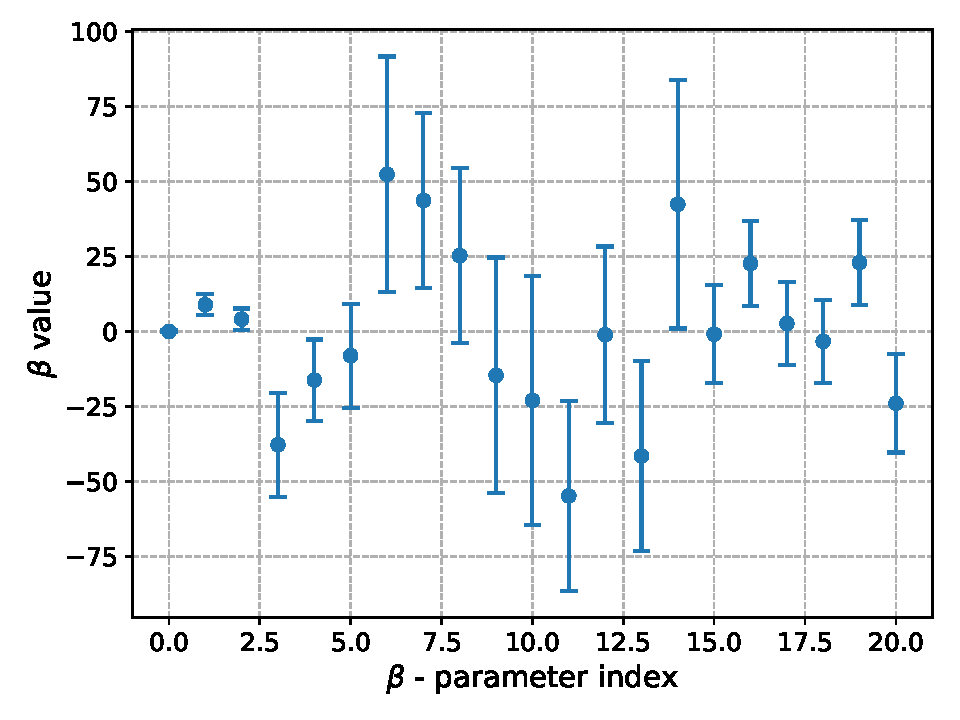
\includegraphics[scale=0.7]{a_CI_betaOLS.pdf}
	\caption{The values of the parameters $\beta$ found from an Ordinary Least Squares fitting, are shown on the $y$-axis, while the index of the parameters are on the $x$-axis. The errorbars are calculated at 95\% confidence}
	\label{fig:1}
\end{figure}

See a large spread in values, and some very large confidence intervals, some spanning from negative to positive values.

MSE score of $4.09\cdot 10 ^{-3}$, and $R^2$ score of $9.50\cdot10^{-1}$

Want a low MSE, and a $R^2$ score close to 1.

Same result using sklearn

\subsection{b) Resampling}
Implement $k$-fold cross validation (CV). We use $k=5$, and our test set is $\frac{1}{5}$ of the full dataset.

When calculating MSE using $mean(y_\mathrm{true}-\tilde y)$,
MSE = $4.62\cdot 10^{-3}$, should do, when we know the true function as we do know. $R^2= 0.944$

Assuming we did not know the true underlying function, and we use our noisy model instead,
MSE = $1.19$

which should be the irreducible noise, that is, $\sigma^2$, which in our case we had chosen as 1.


\subsection{c) Bias-Variance tradeoff}
\subsubsection{1}
Rewrite cost function into bias+variance+irreducible noise
\subsubsection{2}
 Figure similar to Fig. 2.11 of Hastie, Tibshirani, and Friedman
 , which shows the test and training error as a function of the complexity of the model. In our case, the complexity is the polynomial degree.
 
 To reproduce this figure, we will pretend we do not know the true model, and use the noisy data alone. We then get the diagram in Figure \ref{fig:2}. Lowest MSE$= 1.19$ and $R^2=-0.095$
 
 \begin{figure}[H]
 	\centering
 	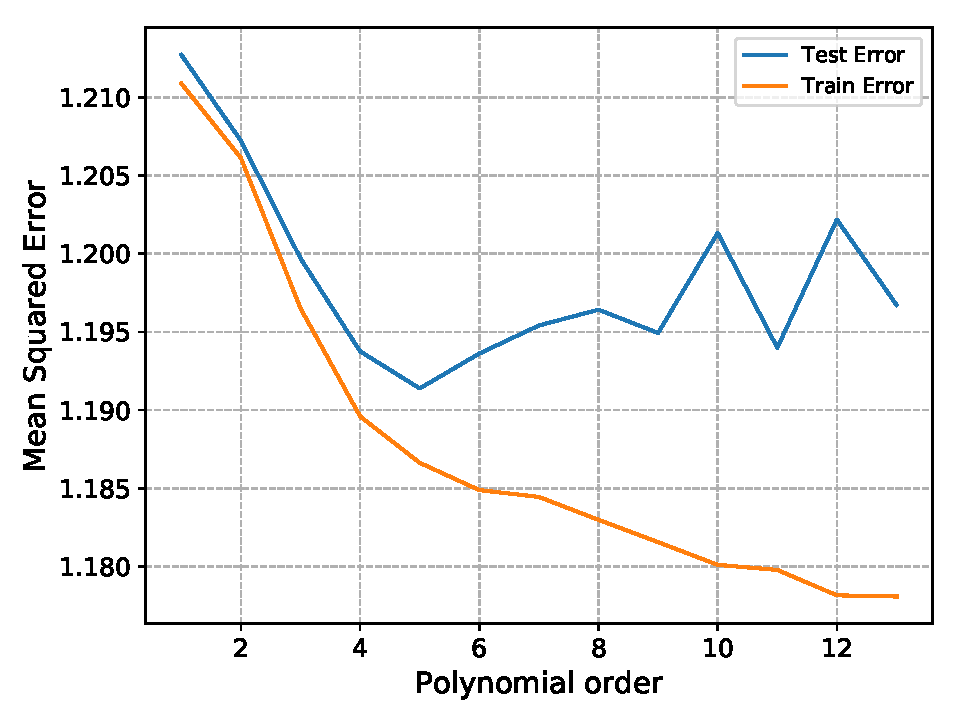
\includegraphics[scale=0.7]{c_OLSerr_train_test_vs_pdegree.pdf}
 	\caption{The training and test MSE for increasing model complexity, using Ordinary Least Squares and $k$-fold Cross Validation. While the test error reaches a minimum before increasing again, the training error will continuously decrease with increasing complexity.}
 	\label{fig:2}
 \end{figure}

Where the training error start going lower than 1, while the test error becomes larger than 1, is where the model start over-fitting, that is, fitting the noise. READ 2.9 OF HASTIE. INCLUDE BIAS AND VARIANCE PLOT IF TIME

Using the true model instead, Lowest MSE$= 4.51\cdot 10^{-3}$ and $R^2= 0.945$

\subsection{d) Ridge regression}
Perform the same analysis a a)-c).

Start then with fitting a fifth order polynomial to the data. First we must choose a $\lambda$ value. We calculate the MSE for a fifth order polynomial fit, with several values of $\lambda$ and using cross validation. This can be seen in Figure \ref{fig:3}. We find that $\lambda=10^{-3}$ minimizes the MSE.

 \begin{figure}[H]
	\centering
	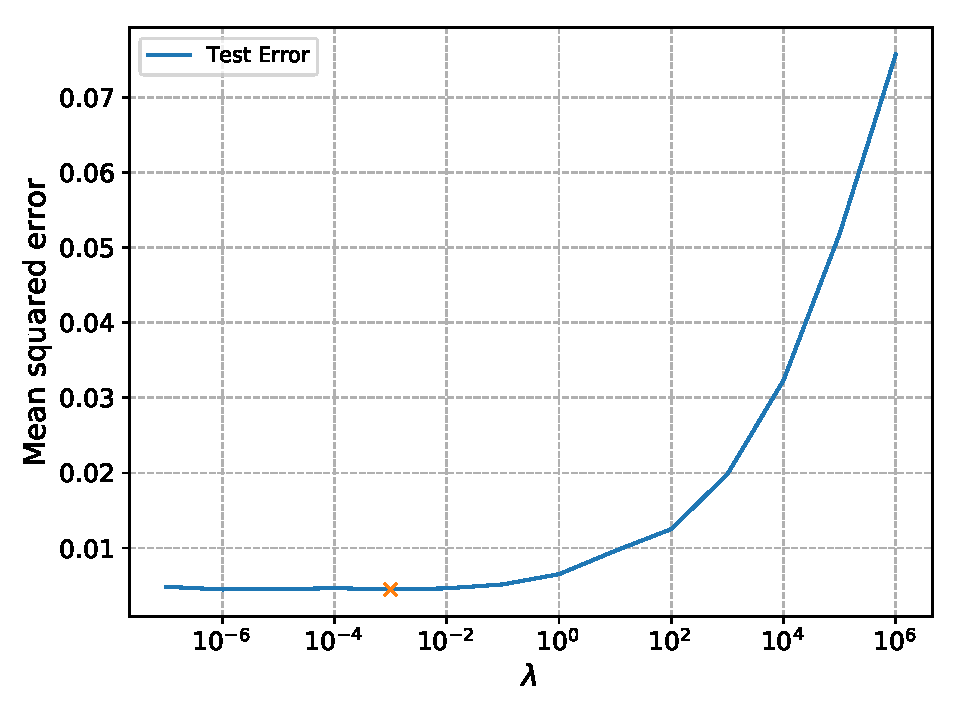
\includegraphics[scale=0.6]{d_lambda_vs_err_d5.pdf}
	\caption{The MSE, calculated using the true model, for the test data for various $\lambda$ values, while using cross validation. The minimum MSE value has been marked by a yellow $\times$.}
	\label{fig:3}
\end{figure}

Without cross-validating, using a fifth order polynomial and $\lambda=10^{-3}$, the MSE score is $4.45\cdot10^{-3}$, and $R^2 = 0.95$

Using resampling, $MSE= 4.51\cdot10^{-3}$, $R^2 =  0.95$.

\begin{figure}[H]
	\centering
	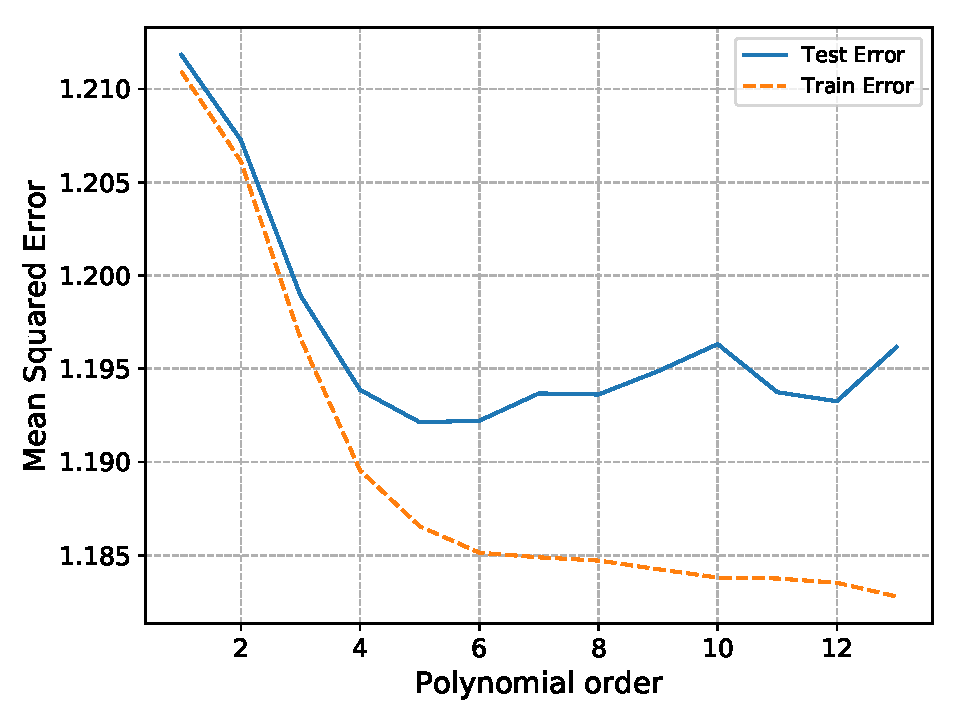
\includegraphics[scale=0.7]{d_Ridge_err_pdegree_noise.pdf}
	\caption{The training and test MSE for increasing model complexity, using Ridge regression and $k$-fold Cross Validation. While the test error reaches a minimum before increasing again, the training error will continuously decrease with increasing complexity.}
	\label{fig:4}
\end{figure}

Calculating MSE as both a function of $\lambda$ and polynomial degree, we get the plot in Figure \ref{fig:5}. According to the figure, a fifth order polynomial which $\lambda=10^{-3}$ fits the data the best, but we see also that the increase in MSE is very small for increasing complexity and $\lambda$ values between $10^{-5}$ to $10^{-1}$.

\begin{figure}[H]
	\centering
	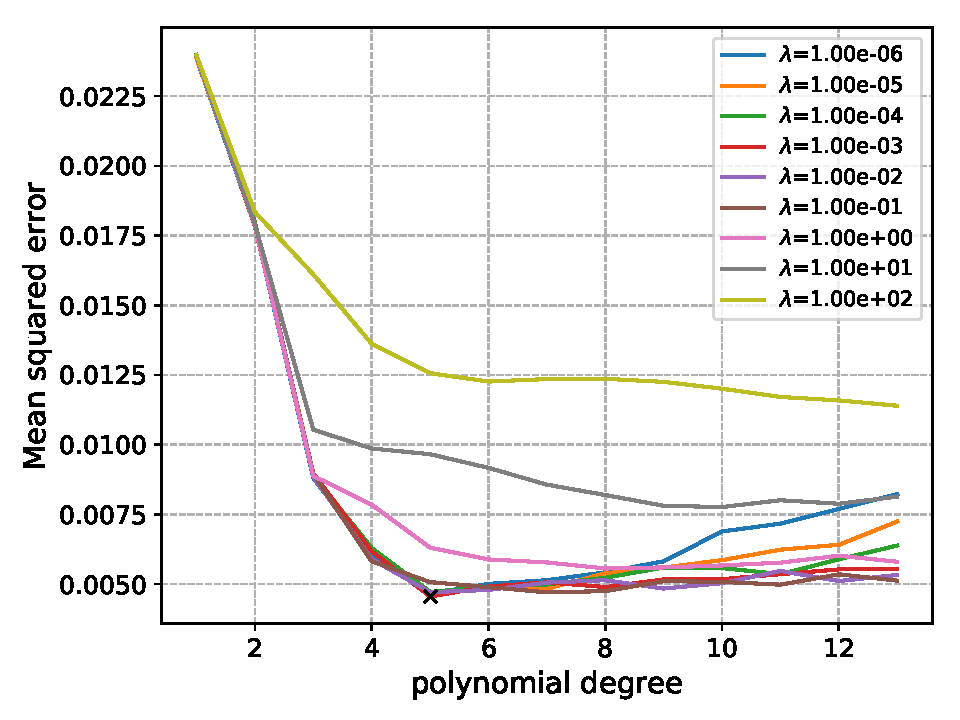
\includegraphics[scale=0.6]{d_Ridge_MSE_pdegree_lmbda.pdf}
	\caption{The MSE, calculated using the true model, for the test data for various $\lambda$ values and polynomial degrees, while using cross validation. The minimum MSE value has been marked by a yellow $\times$.}
	\label{fig:5}
\end{figure}

\begin{figure}[H]
	\centering
	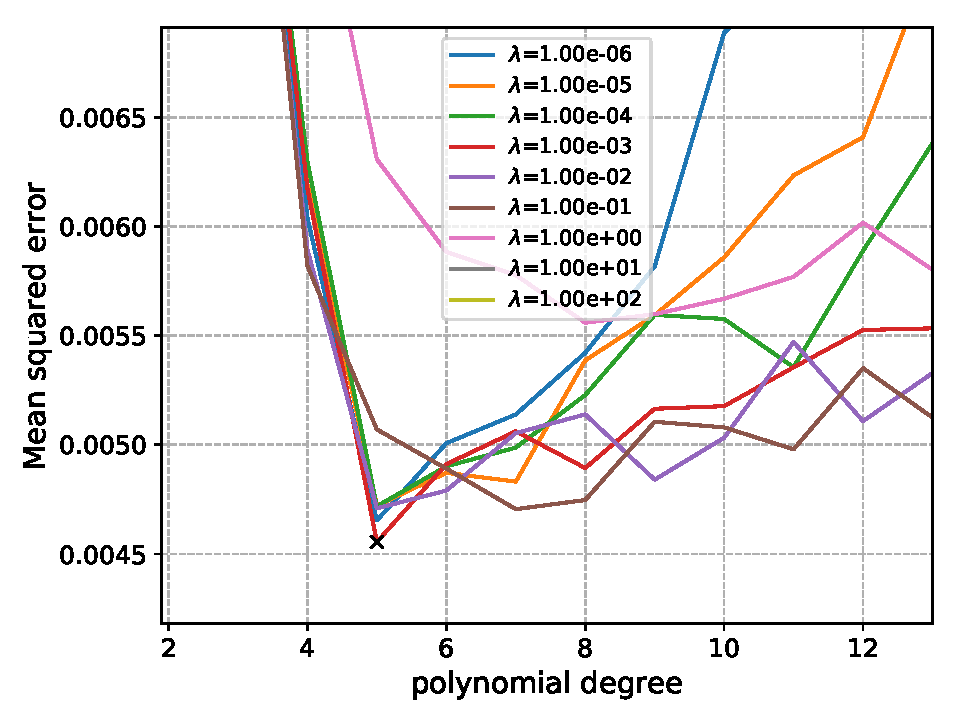
\includegraphics[scale=0.6]{d_Ridge_MSE_pdegree_lmbda_close.pdf}
	\caption{The MSE, calculated using the true model, for the test and training data for various $\lambda$ values, while using cross validation, for a fifth order polynomial. The minimum MSE value has been marked by a yellow $\times$.}
	\label{fig:6}
\end{figure}

\subsection{e) Lasso regression}
Found that $\lambda=10^{-7}$ fit data best, but so does any smaller value, does not seem to stop. $MSE = 4.45\cdot 10^{-3}$
Any $\lambda$ up until $10^{-2}$ does not alter the MSE score much, beyond the fourth decimal.

Found also that fifth degree polynomial fits the data the best, with the same $\lambda$.

Converging issues when calculating for bigger polynomials, so we lowered the $\lambda=10^{-4}$ value, so that the computation time did not take forever. 

Without cross-validating, $MSE=5.46\cdot 10^{-3}$, and $R^2= 0.93$. With noise: $MSE= 1.02$

With cross-validating: $MSE=4.54 \cdot 10^{-3}$, $R^2=0.94$

\section{Discussion}
\section{Conclusion}


\bibliography{library}

\end{document}